\capitulo{2}{Objetivos del proyecto}

Con este proyecto se pretende desarrollar el backend de una futura aplicación móvil, a llamar \emph{RedEM}, focalizada en la experiencia de enfermar para personas afectadas por la EM constituyendo un mapa de autonavegación que les permita hacer uso del sistema sanitario y autogestionar su patología.

Para ello, se plantean los siguientes objetivos funcionales mínimos que el backend a desarrollar deba cumplir:

\section{Objetivos generales}

\begin{itemize}
    \item Ser eficiente y eficaz para el procesamiento y manipulación de datos.
    \item Presentar una sólida, coherente y confiable lógica de negocio. 
    \item Ponderar la seguridad, privacidad e integridad de la información sensible que los usuarios comparten.
    \item Permitir una robusta escalabilidad y rendimiento del sistema.
    \item Permitir que el sistema se integre con servicios internos y externos tales como APIs.
    \item Habilitar un monitoreo y un registro de errores que haga al sistema tolerante a fallos. 
\end{itemize}

\section{Objetivos personales}
\begin{itemize}
\item incluir un chatbot que permita visualizar el funcionamietno de la api por la complejidad 
    \item Incorporar los conceptos fundamentales y aplicaciones del lenguaje de programación Golang para el desarrollo de APIs.
    \item Comprender el funcionamiento de los servidores web y cómo desplegar proyectos desarrollados con el lenguaje Golang.
    \item Aprender a diseñar e implementar APIs RESTful acorde a los estándares de la industria y los principios de escalabilidad.
    \item Adquirir conocimientos sobre el manejo de bases de datos y sistemas de almacenamiento en la nube, y cómo realizar las integraciones con el backend de una aplicación móvil.
    \item Profundizar en el conocimiento de tecnologías y herramientas relacionadas con la seguridad de aplicaciones móviles y servidores.
    \item Robustecer el conocimiento en cuanto al uso de sistema de control de versiones Git, a través de la plataforma GitHub, para trabajar de manera eficiente en proyectos de desarrollo de software en equipo.
   \item Aprehender a utilizar software para la planificación y ejecución del trabajo de desarrollo de software mediante el uso de la metodología SCRUM.
    \item Conocer cómo utilizar el procesador de textos \LaTeX\ para la creación de documentos técnicos y científicos de alta calidad, como la memoria del presente proyecto.   
\end{itemize} 

\newcommand{\graybox}[2]{%
    \colorbox{gray!20}{%
        \parbox{\dimexpr\linewidth-2\fboxsep}{%
            \colorbox{black}{\textcolor{white}{\textbf{\makebox[\dimexpr\linewidth-2\fboxsep]{#1}}}}\vspace{4pt}%
            \hspace{\parindent}#2%
        }%
    }%
}

\graybox{A considerar:}{\\Debido a que el TFG pondera únicamente el desarrollo del backend, no así de la aplicación \emph{RedEM}, la visibilidad o testing del proyecto queda restringida. \\Por tal motivo se emplea la plataforma Postman para que el comité evaluador se sirva probar el funcionamiento de las APIs, tanto del backend como del chatbot, conforme figura en el Manual de Usuario. \\
Amerita explicitar, además, que para las APIs de backend los datos son ficticios, mientras que en el caso del chatbot, la información es extraída del sitio web de la Asociación.}



            



\section{Análisis de mercado}
Para la creación del presente proyecto se consideró la posible existencia de otras aplicaciones de similares características a nivel global. Por tanto, en este apartado se expondrá información relativa a: población objetivo, competencia y antecedentes, y análisis FODA en base a la información relevada.

\subsection{Público objetivo y perfiles de usuario}
\emph{RedEM} es una aplicación dirigida a los principales grupos afectados e involucrados en la EM, que sería: personas con EM, allegados y familiares, personal sanitario de carácter multidisciplinar.

\begin{itemize}
    \item 
    \textbf{Personas con EM:} Los pacientes presentan una amplia gama de síntomas que pueden variar de un individuo a otro tanto en frecuencia, como en tipo e intensidad. En tal sentido, cada paciente tendrá una serie de necesidades diferentes requiriendo un tratamiento y seguimiento particular, lo que debe ser considerado dentro del diseño de la aplicación móvil y su usabilidad.
    \item 
    \textbf{Allegado y familiares:} Ante el diagnóstico de EM, el entorno del paciente se ve afectado, en especial aquellas personas que asumen el rol de cuidadores. Éstos tienen, a su vez, una serie de necesidades que también debe ser cubiertas o que ameritan una solución, como por ejemplo: consejos para el cuidador del paciente, primeros auxilios en caso de emergencia, apoyo emocional, o cualquier otra necesidad que pueda surgir.
   \item 
   \textbf{Personal sanitario multidisciplinar:} Por ser una enfermedad neurológica que afecta el funcionamiento del sistema nervioso central, puede generar síntomas funcionales y estructurales que repercuten en diversas áreas del organismo siendo imprescindible un abordaje integral con la participación de diversos especialistas como ser: neurólogos, fisioterapeutas, terapista ocupacional, psicólogos, sexólogos, entre otros.  
\end{itemize} 


\subsection{Competencia/Antecedentes}
Existen diversas aplicaciones que buscan ayudar a potenciar la autonomía personal de los pacientes con EM. No obstante, la mayoría de ellas se centran en consejos y ejercicio físicos, más no tienen en cuentan la comunicación con especialistas ni el control y seguimiento de la enfermedad y su tratamiento. A este respecto, el análisis de la competencia se enfocó en la búsqueda de aplicaciones que cumplieron con el objetivo del presente proyecto para, posteriormente, compararlas con \emph{RedEM}. A continuación, se describen las cuatro aplicaciones que se encontraron:

\subsubsection{Cleo}
Cleo es una app móvil, para iOS y Android, desarrollada por la compañía Biogen, y cuyo objetivo es brindar acompañamiento a los pacientes de EM. Para ello le permite a los usuarios establecer diálogos directos, mediante chats, con servicios de enfermería especializados con la EM para resolver dudas o solicitar apoyo, al mismo tiempo que proporciona otras herramientas como contenido de valor en forma de consejos, noticias y artículos con información de interés.

\begin{figure}[h]
    \centering
    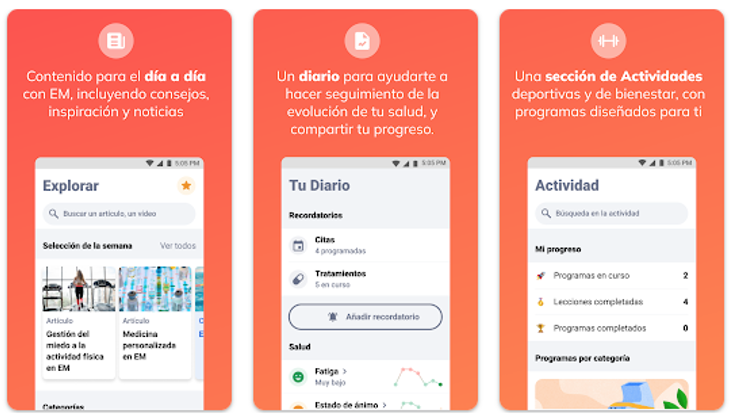
\includegraphics[width=0.7\textwidth]{img/mercado/cleo.png}
    \caption{Cleo App.} \label{Img:Cleo+App}
\end{figure} 

Por otro lado, también dispone de un diario para llevar un control y registro de la salud del paciente, los síntomas que ha presentado a lo largo del día, y su estado de ánimo, que luego pueda compartir con el personal sanitario. Asimismo, propone planes de ejercicio físico adaptado, y un sistema de alarmas y recordatorios para citas médicas y tratamientos.

A pesar de sus bondades, esta aplicación no permite ser descargada en Latinoamérica y, al tratarse de una herramienta digital creada por una farmacéutica, los datos allí cargados terminan siendo propiedad de la misma.

\subsubsection{ME - Multiple Esclerosis}

ME es un app móvil disponible en iOS y Android, desarrollada por Novartis. Su objetivo principal en facilitar el seguimiento y control de los síntomas del paciente, para lo cual cuenta con tres funciones básica. La primera de ellas, un plan de ejercicios diseñado para optimizar la movilidad y capacidad cognitiva.

Luego, la aplicación cuenta con una sección para el registro de datos diarios, semanales o mensuales, referentes a las consultas médicas y horarios de tratamiento, en la que podrán también configurar alarmas y recordatorios; y un cuerpo humano interactivo en el que el usuario podrá indicar las partes de su cuerpo donde presenta síntomas. Por otra parte, sirve también de apoyo al personal de salud quienes podrán llevar un seguimiento a partir de la información recogida por la app.

\begin{figure}[h]
    \centering
    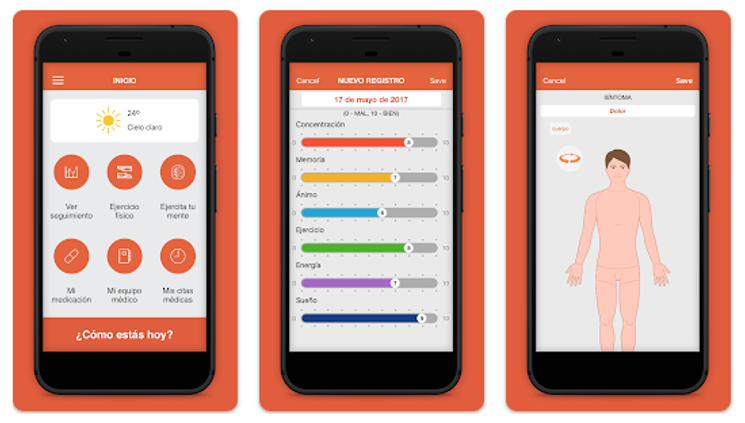
\includegraphics[width=0.5\textwidth]{img/mercado/me.png}
    \caption{ME App} \label{Img:ME+App}
\end{figure} 

Tal como en el caso anterior, está aplicación no puede ser descargada en la región y los datos son propiedad de una empresa farmacéutica. 

\subsubsection{Control EM}

Si bien no fue posible acceder en la actualidad a esta aplicación ni descargarla en la región, en tanto antecedente amerita mencionarla. Control EM era una aplicación para iOS, desarrollada por la Fundación Esclerosis Múltiple Madrid (FEMM) y que, al igual que las anteriores, buscaba ayudar a los pacientes a llevar un control de su enfermedad, su evolución, disponer de información de interés y comunicarse con especialistas. 

\begin{figure}[h]
    \centering
    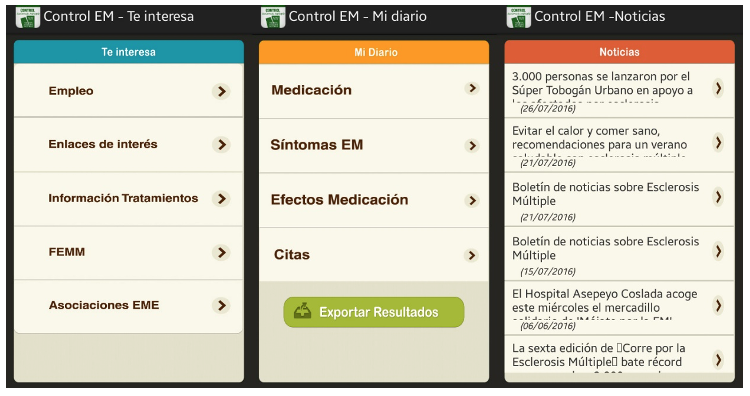
\includegraphics[width=0.5\textwidth]{img/mercado/control_em.png}
    \caption{Control EM App} \label{Img:Control+EM+APP}
\end{figure} 

Contaba con cuatro secciones principales: a) mi diario, en donde el usuario podía anotar su horario de tratamiento, síntomas, efectos de la medicación y citas médicas, para así conocer su evolución a través de gráficas; b) agenda, donde se mostraban las citas anuales vinculadas con la EM, como conferencias; c) noticias, donde se brindaba información sobre la EM; y d) te interesa, que incluía información sobre tratamientos disponibles, empleo, taxis adaptados, y contactos de la FEMM u otras asociaciones.

\subsubsection{Emilyn}

Al igual que el caso anterior, Emilyn sirve como antecedente a nuestros propósitos ya que no fue posible encontrarla activa. Esta aplicación funcionaba como una compañera digital para la persona con EM, permitiéndole llevar un control y registro de los síntomas, crear alertas y recordatorios para la medicación y las citas médicas, guardar y compartir informes médicos, o descubrir potenciales desencadenantes de empujes. Esta aplicación sólo estaba disponible en inglés y no se encontraba habilitada para la región.

\begin{figure}[h]
    \centering
    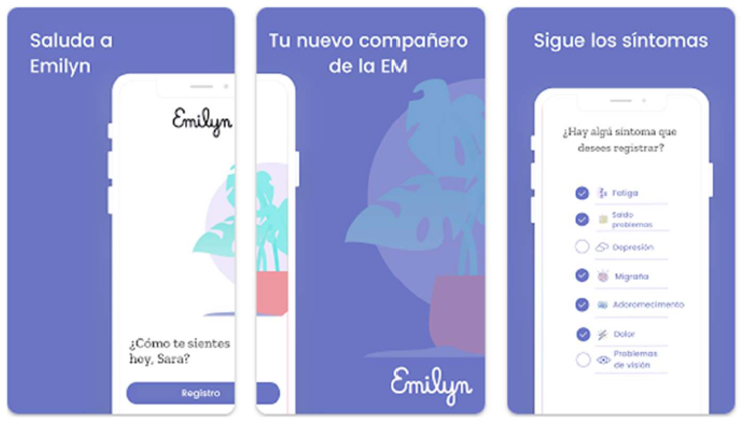
\includegraphics[width=0.5\textwidth]{img/mercado/emylin.png}
    \caption{Emylin App} \label{Img:Emilyn+APP}
\end{figure} 

\subsection{Discusión del estado de mercado para los objetivos del proyecto}
Habiendo analizado las aplicaciones existentes en el mercado que se acercan al objetivo planteado y a las necesidades del presente proyecto, se procede a formular un análisis FODA al respecto de \emph{RedEM}.

\subsection{Análisis FODA}

\begin{tabular}{|c|l|}
\hline
\textbf{Fortalezas} & \parbox{10cm}{
\begin{itemize}
    \item Aplicación gestionada por una organización civil y no la industria farmacéutica, por lo que se erradican conflictos de interés actuales o potenciales.
    \item Contribuye a la creación de un mapa de autonavegación a partir de información proporcionada por la sociedad civil organizada (live-experience), desde una perspectiva holística y multidimensional.
    \item Ofrece al usuario información referida a dispositivos y programas disponibles en la matriz de protección social, asi como recetas alimenticias, sección de preguntas y respuestas, y estado del clima para el cuidado del paciente, en formato de artículos.
    \item El frontend se desarrollará en lenguaje Flutter para permitir ahorrar costos de desarrollo por concepto de portabilidad de código.
    \item El chatbot con IA es algo novedoso y que permite descongestionar la atención telefónica que brinda la Asociación EMUR.
\end{itemize}
} \\
\hline
\textbf{Oportunidades} & \parbox{10cm}{
\begin{itemize}
    \item Permite que los pacientes estén interconectados para sobrellevar la enfermedad, generando comunidad.
    \item La mayoría de la población uruguaya cuenta con smartphones con acceso a internet.
    \item A nivel país se tiene un estable acceso a internet debido a que se cuenta con la infraestructura para ello. 
    \item Tiene potencial para ser replicable y escalable a otras patologías así como también a otros contextos socio-económicos, culturales y geográficos.
    \item Auge de la telemedicina, así como de iniciativas de recolección de resultados y experiencias aportadas por los pacientes (PROMs y PREMs).
\end{itemize}
} \\
\hline
\end{tabular}

\begin{tabular}{|c|l|}
\hline
\textbf{Debilidades} & \parbox{10cm}{
\begin{itemize}
    \item Aún no permite establecer contacto directo con el personal sanitario mediante chat.
    \item La Asociación es pequeña para administrar los contenidos de la aplicación, por lo que requerirá un equipo de gestión de contenidos.
    \item Al tratarse de una Asociación de exiguos ingresos, será un desafío asumir a largo plazo los costos de mantenimiento y difusión.
\end{itemize}
} \\
\hline
\textbf{Amenazas} & \parbox{10cm}{
\begin{itemize}
    \item Baja adopción por parte de los usuarios, debido a que Uruguay presenta una población mayoritariamente envejecida y existe fuga de cerebros.
    \item Aplicaciones de la industria farmacéutica que puedan desarrollarse en la región próximamente, o que sean adaptadas para Latinoamérica. 
    \item Cambios respecto a la normativa vigente en cuanto al uso de datos personales.
\end{itemize}
} \\
\hline
\end{tabular}





